\chapter{Chrome擴充套件設計}
\indent
在撰寫網頁測試腳本時,
為了避免網頁改版後,腳本內部中專門定位內部元件的Xpath無法正確抓取元件位置,導致腳本頻頻出錯,
專門定位網頁中元件的Xpath表達式就必須越穩定越好。
使用越穩定的表達式相對來說需要設定很多限制條件,尋找符合的限制條件對測試人員會是需要一定的經驗且較花時間的事情。
本論文以呂昭陞論文中提出提升穩定性的Xpath撰寫樣式為基礎,
提出在測試人員需要找尋適合的條件的時候可以透過Chrome擴充套件增加比較HTML文檔和過濾自訂屬性...等等額外功能的設計,
讓使用者即使在大型架構的HTML中也可以減少對於測試人員屬於雜訊的元件,可以較快速的挑選出想要屬性來設定適合的條件,
來撰寫適合定位該元件的Xpath表達式。

% =========================================================================================
% =========================================================================================
\section{系統架構}\label{s3.1}
圖\ref{f3.1}為為Chrome擴充套件實作的系統架構圖,下列為各元件之介紹:

\begin{itemize}
\item\textbf{Chrome:}
以市占率第一的Chrome瀏覽器為背景下,對瀏覽器擴充元件進行實作

\item\textbf{Chrome Extension:}
對Chrome瀏覽器加裝此擴充功能之擴充程式

\item\textbf{Content Script For Extension:}
擴充程式腳本之一, 用來在瀏覽器網頁上執行的JavaScript程式,可讀取該網頁的資訊並操作或傳給擴充元件

\item\textbf{Background Script For Extension:}
擴充程腳本之一, 屬於擴充元件的背景程序,通常會將程式的主要邏輯放在此腳本中

\item\textbf{SidePanel Script For Extension:}
擴充程式腳本之一, 在擴充元件Element頁面下的子頁面

\item\textbf{HTML Compare Function:}
比對兩個HTML差異之程式模組

\item\textbf{UI Interface:}
擴充元件在SidePanel裡面的使用者介面設計

\item\textbf{Test Script:}
針對Compare Function的單位測試腳本

\end{itemize}

\begin{figure}[H]
    \centering
    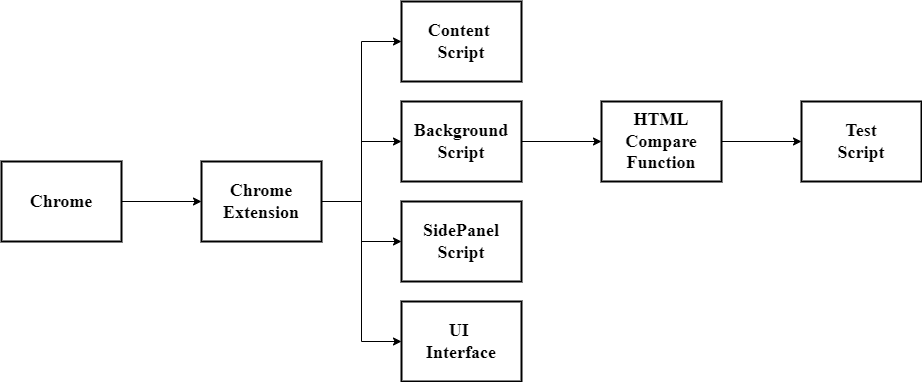
\includegraphics[width=0.9\textwidth]{picture/ch3-systemStucture.png}
    \caption{擴充元件實作之架構圖}
    \label{f3.1}
\end{figure}

此設計架構主要是以HTML比對函數為主,利用Chrome Extension的專用腳本們,把網頁的HTML讀取後丟入該比對系統,
比對完再進行回傳動作,最後利用UI介面把結果顯示在畫面上。

% =========================================================================================
% =========================================================================================
\section{HTML比對之實作}\label{s3.2}
\indent

若確定要開始進行比對網頁中的HTML文本後,需要先取出先前和之後的兩個HTML文本,然後進行文本前後比對。
此比對功能,使用了開源程式Hiff的架構,經過權重部分修改、輸出元件的調整以及增加相關測試腳本,調整成
適合擴充程式的內部核心程式。圖\ref{f3.2}為HTML比對之活動圖

\begin{figure}[H]
    \centering
    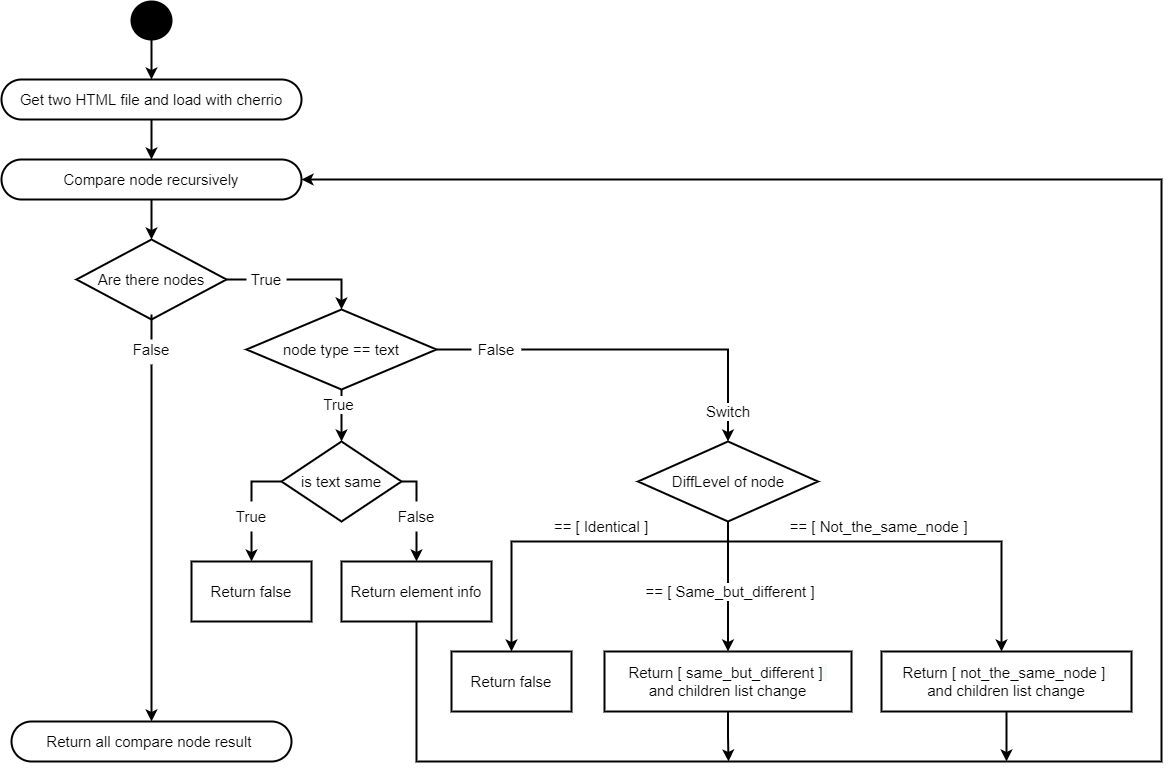
\includegraphics[width=1.0\textwidth]{picture/ch3-activity diagram.png}
    \caption{HTML比對之活動圖}
    \label{f3.2}
\end{figure}

\subsection{判斷節點相異程度}\label{s3.2.1}
在兩節點相互比對後,需要有一個判斷方法來確定該節點的相異程度,會分成三個等級:Identical、Same but different和Not the same node。
本程式的實作流程為圖\ref{f3.3},會先做比各屬性的比對,然後根據當前狀況選擇要該屬性自定義的權重,最後將所有權重相加來節點判斷相異等級

\begin{figure}[H]
    \centering
    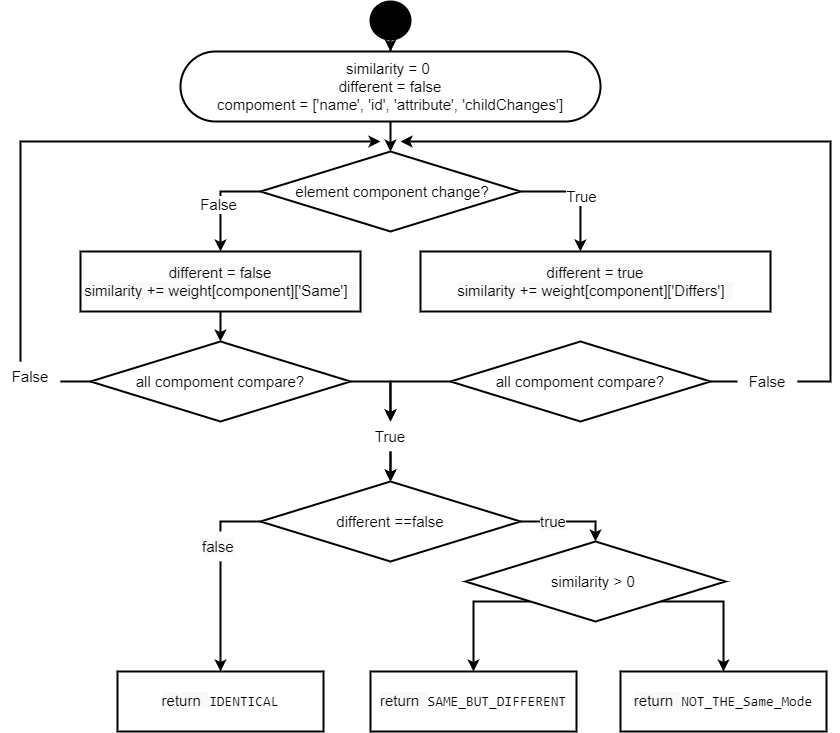
\includegraphics[width=1.0\textwidth]{picture/ch3_HEURISTIC_comapre.png}
    \caption{節點相異程度之活動圖}
    \label{f3.3}
\end{figure}

\subsection{比對輸出結果}\label{s3.2.2}
在比對的時候有分成三種類型:Changed、Added和Removed,三種類型需要回傳相對應的資訊,
舊有的程式庫僅只有對該變更資訊用最低限度的字串來表示變更,經過修改後,將輸出結果加上變更節點的解析結果以及詳細屬性變化資訊,
在顯示上可以將結果直接輸出在畫面上,減少其他額外的處理。

在程式碼\ref{l3.1}為changed類型的輸出結果,
其中除了回傳相關的解析後的節點資訊,
裡面"info-compare"的值為比對該變化元件的所有類別結果,包括比對前、比對後和差異結果。

\begin{lstlisting}[caption=比對輸出結果(changed類型), label={l3.1}]
    1   function changed($nodeBefore, $nodeAfter) 
    2   {
    3    var before = grabParentAndIndex($nodeBefore),
    4    after = grabParentAndIndex($nodeAfter);
    5
    6    return {
    7    type: "changed",
    8    before:locationInfo(before.$parent, $nodeBefore, before.index),
    9    after: locationInfo(after.$parent, $nodeAfter, after.index),
    10   selectingNode: $nodeAfter,
    11   nodeINFO: $nodeBefore,
    12   info-compare: info_compare ($nodeBefore, $nodeAfter)
    13   };
    14  }
\end{lstlisting}

在程式碼\ref{l3.2}和程式碼\ref{l3.3}為added和changed類型的輸出結果,
其中除了回傳相關的解析後的節點資訊,
裡面"icontentHTML"的值為added或removed元件的內部HTML資訊,會在UI介面中將整個變更的區塊告訴使用者。

\begin{lstlisting}[caption=比對輸出結果(added類型), label={l3.2}]
    1   function added($addedNode, $parentBefore, indexBefore, 
    2       $parentAfter, indexAfter) 
    3   {
    4     return {
    5     type: "added",
    6     before: locationInfo($parentBefore, undefined, indexBefore),
    7     after:  locationInfo($parentAfter, $addedNode, indexAfter),
    8     selectingNode: $parentAfter,
    9     nodeINFO: $addedNode,
    10    contentHTML: stringify($addedNode, false),
    11    };
    12  }
\end{lstlisting}

\begin{lstlisting}[caption=比對輸出結果(removed類型), label={l3.3}]
    1   function removed($removedNode, $parentBefore, indexBefore, 
    2       $parentAfter, indexAfter) 
    3   {
    4    return {
    5    type: "removed",
    6    before: locationInfo($parentBefore, $removedNode, indexBefore),
    7    after:  locationInfo($parentAfter, undefined, indexAfter),
    8    selectingNode: $parentAfter,
    9    nodeINFO: $removedNode,
    10   contentHTML: stringify($removedNode, false),
    11   };
    12  }
\end{lstlisting}


% =========================================================================================
% =========================================================================================
\section{擴充元件腳本設計之實作}\label{s3.3}
\indent
在章節\ref{s2.6.3}有對不同類型的腳本做基本介紹,針對各腳本獨特的特性分配它需要執行的功能。
圖\ref{f3.4}中表示出執行功能後的執行順序及流程,從按下比對文本的按鈕到比對結束的內部腳本們的流程圖。

\indent

\begin{figure}[H]
    \centering
    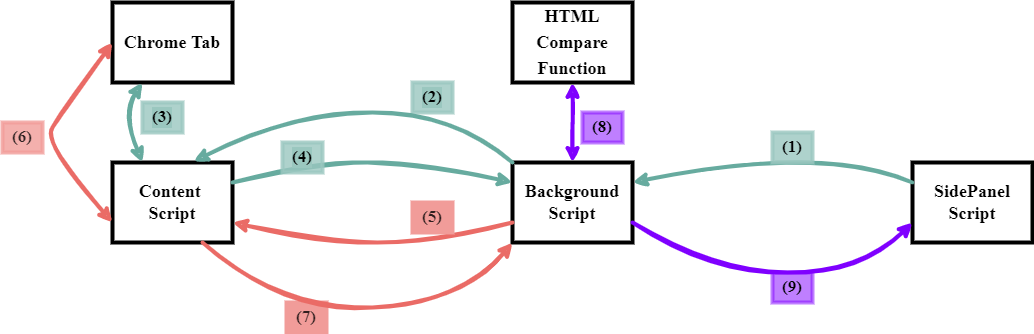
\includegraphics[width=1\textwidth]{picture/ch3-script-structure.png}
    \caption{extension script}
    \label{f3.4}
\end{figure}

\subsection{SidePanel Script}\label{s3.3.1}
SidePanel Script是專門控制在Chrome Developer tools中Elements頁面中旁邊子介面的腳本,
此腳本主要功能在於若使用者點擊畫面中的互動按鈕或輸入相關字元,會讓擴充元件開始做動。
圖\ref{f3.4}的起始點是從此腳本開始的,
在UI介面下點擊開始比對的按鈕使開始與Background Script溝通後讓他知道要開始要進行比對了,
最後等到比對完後從Background Script得到結果並且把結果顯示在UI介面上。

\subsection{Background Script}\label{s3.3.2}
Background Script在擴充元件中的定位是在背景中執行的程式,開發者通常將此程式的主要邏輯撰寫在這腳本中,
而HTML比對腳本的函數也是在此腳本中執行的,在執行前會先等待比較前的HTML文本先傳遞到此並等待Timer時間,
若時間到了則會繼續再去取得當下的HTML文本,最後再進執行HTML Compare函數的文本比較,最後回傳到SidePanel Sdcript中。
圖\ref{f3.4}中的Background Script主要是集中在與Content Script溝通來取出HTML文本,最後再執行比對並回傳。

\subsection{Content Script}\label{s3.3.3}
若要訪問網頁的資訊或者是直接新增或刪除當下的DOM結構,則必須要透過Content Script來執行相關的程式碼。
在進行與內容腳本通訊時,要找到當下頁面的Tab Id才可以進行正確的溝通,
成功建立溝通的管道後,即可以透過此腳本取出HTML文本並將結果回傳給Background Script來執行比對函數。
圖\ref{f3.4}中的Content Script主要負責的是當前的Chrome Tab取出HTML文本回傳給Background Script提共比對資料。

\section{UI/UX介面之實作}\label{s3.4}
設計此工具,為考慮人性化的使用介面以及比對後的結果方便使用者挑選所需要的條件,將此工具分成以下五個部分:
\begin{itemize}
    \item\textbf{Illustrate:}
    
    說明此擴充工具功能並且敘述該工具選擇的設定方式以及使用流程。

    \item\textbf{Timer:}
    
    依照使用者當前的網路狀況、元件互動情況...等等因素來調整前後HTML中間的比較時間
    
    \item\textbf{Options:}
    
    針對當前使用者狀態,透過選擇對應狀況的選項,讓使用者可以過濾掉大多數不需要的結果
    \begin{itemize}
        \item\textbf{Ignore style attribute's change}
 
        在HTML文件樣式中,有時會利用<style>標籤來建立簡易的CSS指令,但通常在使用時,較少用此標籤來設定條件,
        為避免有很多節點因為style屬性變化,造成比對結果較多不必要的資訊,故設立此條件來篩選。

        \item\textbf{Only display change of current selecting elemnt}
        
        若當前的HTML文本結構過大,但使用者僅僅只是要查看當前節點的變化,過多的變更結果會讓使用者較難找到適合當下情況的條件,
        為過濾掉當前節點之外的變更雜訊,在develope tool中Element頁面點擊HTML的節點,比較後的顯示結果僅會出現該節點的變化結果。
        
        \item\textbf{Display one tag's change}
        
        為避免比較後的結果過多,故添加了過濾元件tag的選項,
        讓使用者可以利用節點的tag過濾比對後的結果,例如:div、button...等等類別。
    \end{itemize}
    
    \item\textbf{Compare Control:}
 
    內部有兩個按鈕以及顯示比較情況的顯示框,可以點擊按鈕開始比對或典籍按鈕強制停止比對
    
    \item\textbf{Compare Result:}

    此面板中的下拉選單有顯示三中累行的結果:changed-area、added-area和removed-area,點擊後會出現表格顯示該節點的屬性比對,
    內部表格顯示該節點所有屬性的before、after和diff比對結果
    
    \end{itemize}
\indent

\begin{figure}[H]
    \centering
    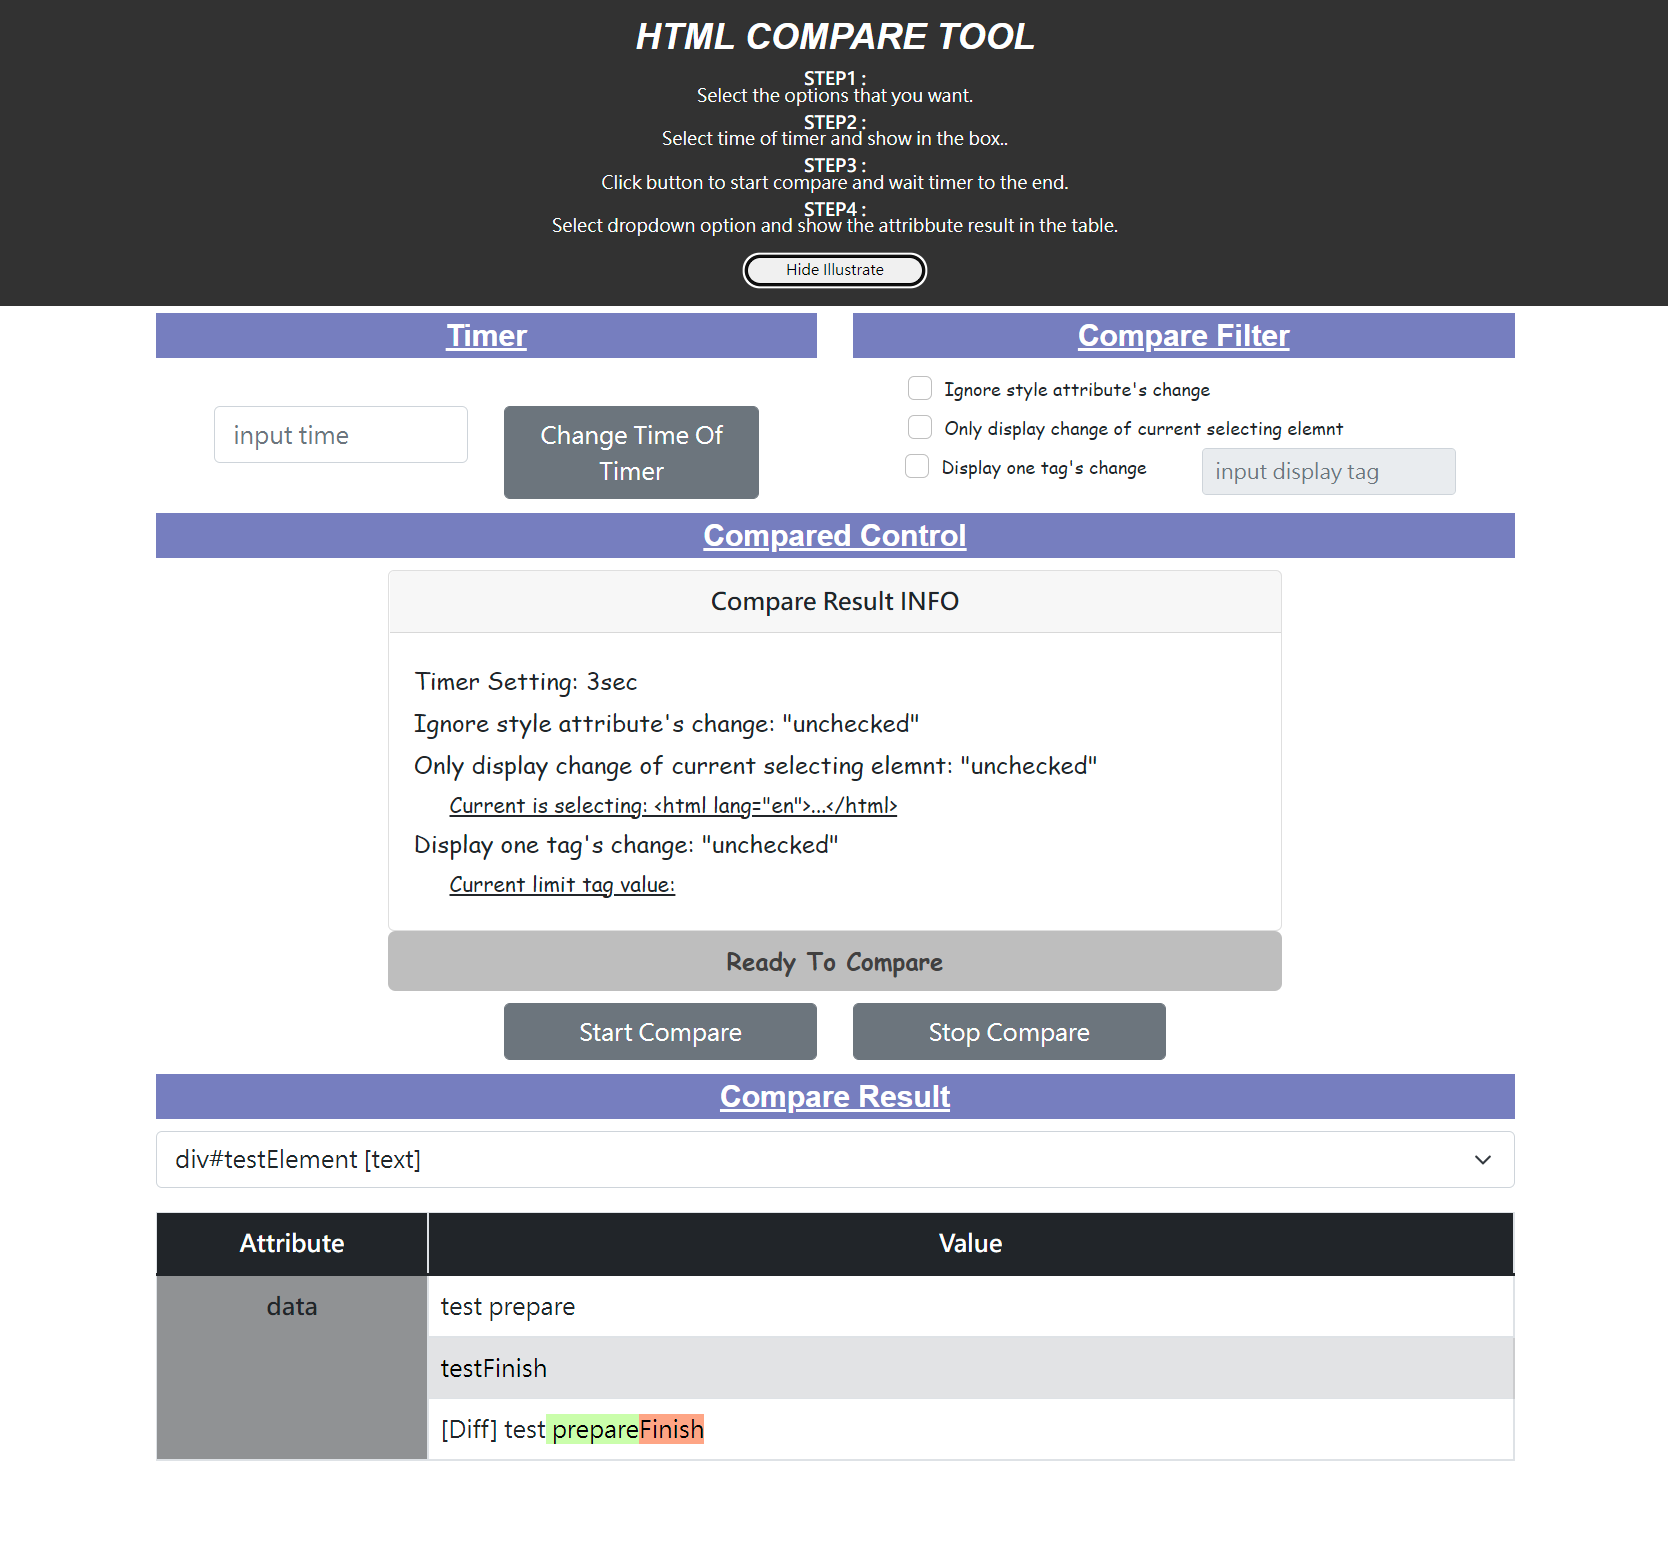
\includegraphics[width=1\textwidth]{picture/ch3-UIUX-example.png}
    \caption{UI設計之介面}
    \label{f3.5}
\end{figure}